\chapter{Extraction Method Based on Manually Created Rules} \label{sec:ch50_manual_rules_chapter}
\graphicspath{{../img/ch50/}}

%%%%%%%%%%%%%%%%%%%%%%%%%%%%%%%%%%%%%%%%%%%%%%%%%%%%%%%%%%%%%%%%%%%%%%%%%%%%%%%%%%%%%
\section{Introduction}
%%%%%%%%%%%%%%%%%%%%%%%%%%%%%%%%%%%%%%%%%%%%%%%%%%%%%%%%%%%%%%%%%%%%%%%%%%%%%%%%%%%%%

\subsection{Presented Extraction Methods}

The main motivation for creating both these methods was an attempt to use deep linguistic analysis of natural language texts. Especially for the Czech language with free word order this seemed reasonable. It is much more straightforward to design extraction rules on the basis of linguistic dependency trees than to struggle with the surface structure of text. In a dependency tree a position of a word is determined by its syntactic (analytical trees) or even semantic role (tectogrammatical trees). So the extraction rules might not be dramatically affected by minor variations (not changing the factual meaning of a sentence) of the word order.







%%%%%%%%%%%%%%%%%%%%%%%%%%%%%%%%%%%%%%%%%%%%%%%%%%%%%%%%%%%%%%%%%%%%%%%%%%%%%%%%%%%%%
\section{Implementation}
%%%%%%%%%%%%%%%%%%%%%%%%%%%%%%%%%%%%%%%%%%%%%%%%%%%%%%%%%%%%%%%%%%%%%%%%%%%%%%%%%%%%%

\subsection{Procedural Extraction Rules} \label{sec:ch50_Procedural_Extraction_Rules}

Our first implementation was based on Btred API for processing linguistic trees. The extraction rules were implemented as Perl Btred procedures that were evaluated on all of the trees of an arbitrary corpus by Btred. An example of such extraction rule is in Figure~\ref{lst:btred_rule} and corresponding extraction output on Figure~\ref{fig:btred_xml}.


%%%%%%%%%%%%%%%%%%%%%%%%%%%%%%%%%%%%%%%%%%%%%%%%%%%%%%%%%%%%%%%%%%%%%%%%%%%%%%%%%%%%%
\begin{figure}
\begin{minted}[linenos,  fontsize=\footnotesize,
               frame=lines]{perl}
#variable $this contains currently processed node, $root current root node

my @injure_verbs = ("zranit", "usmrtit", "zemřít", "zahynout", "přežít");

sub print_injured {
	if ($this->{gram}{sempos} eq "v") {
		foreach my $v (@injure_verbs) {
			if ($this->{t_lemma} eq $v ) {
				#action type
				print "<action type=\"" . $this->{t_lemma} . "\">";

				#sentece
				print "<sentece>" . PML_T::GetSentenceString($root) . "</sentece>";
				print "<sentece_id>" . $root->{id} . "</sentece_id>";
				
				#negation
				if (test_negation($this)) {
					print "<negation>true</negation>" ;					
				} else {
					print "<negation>false</negation>" ;										
				}
								
				#manner of injurance
				my @mans = find_node_by_attr_depth($this, 0, 'functor', '^MANN');
				if (@mans) {
					foreach my $m (@mans) {
						print "<manner>"; 
						print $m->{t_lemma};
						print "</manner>"; 
					};
				}
				
				#actors and patients
				my @pats = find_node_by_attr($this, 'functor', '^[PA][AC]T');
				@pats = &filter_list(\&test_person, @pats);
				
				foreach my $p (@pats) {
					print "<participant type=\"" . $p->{t_lemma} . "\">";

					#patients count
					my @cnt = find_node_by_attr($p, 'functor', '^RSTR');
					@cnt = &filter_list(\&test_number_lemma, @cnt);
					my $cnt1 = pop(@cnt);
					print "<quantity>" . 
						&test_number($cnt1->{t_lemma}) . 
						"</quantity>" if ($cnt1);
	
					print "<full_string>";
					print_subtree_as_text($p);
					print "</full_string>";

					print "</participant>";
				}
				
				#action end
				print "</action>\n";											
}}}}
\end{minted} 
																																		\begin{comment}
																																		this >>$<< hacks my syntax highlighter :-)
																																		\end{comment}
\caption{Procedurally written extraction rule in \emph{Btred}.}
\label{lst:btred_rule}
\end{figure}
%%%%%%%%%%%%%%%%%%%%%%%%%%%%%%%%%%%%%%%%%%%%%%%%%%%%%%%%%%%%%%%%%%%%%%%%%%%%%%%%%%%%%




%%%%%%%%%%%%%%%%%%%%%%%%%%%%%%%%%%%%%%%%%%%%%%%%%%%%%%%%%%%%%%%%%%%%%%%%%%%%%%%%%%%%%
\begin{figure}
\begin{minted}[linenos,  fontsize=\footnotesize,
               frame=lines]{xml}
<injured_result>
	<action type="zranit">
		<sentece>
			Při požáru byla jedna osoba lehce zraněna -- jednalo se
			o majitele domu, který si vykloubil rameno.
		</sentece>
		<sentece_id>T-vysocina63466.txt-001-p1s4</sentece_id>
		<negation>false</negation>
		<manner>lehký</manner>
		<participant type="osoba">
			<quantity>1</quantity>
			<full_string>jedna osoba</full_string>
		</participant>
	</action>
	<action type="zemřít">
		<sentece>
			Ve zdemolovaném trabantu na místě zemřeli dva muži -- 82letý
			senior a další muž, jehož totožnost zjišťují policisté.
		</sentece>
		<sentece_id>T-jihomoravsky49640.txt-001-p1s4</sentece_id>
		<negation>false</negation>
		<participant type="muž">
			<quantity>2</quantity>
			<full_string>dva muži</full_string>
		</participant>
	</action>
		<action type="zranit">
		<sentece>čtyřiatřicetiletý řidič nebyl zraněn.</sentece>
		<sentece_id>T-jihomoravsky49736.txt-001-p4s3</sentece_id>
		<negation>true</negation>
		<participant type="řidič">
			<full_string>čtyřiatřicetiletý řidič</full_string>
		</participant>
	</action>
</injured_result>
\end{minted}
\caption{\emph{XML} structured output of the query written in \emph{Btred}.}
\label{fig:btred_xml}
\end{figure}
%%%%%%%%%%%%%%%%%%%%%%%%%%%%%%%%%%%%%%%%%%%%%%%%%%%%%%%%%%%%%%%%%%%%%%%%%%%%%%%%%%%%%




\subsection{Netgraph Based Extraction Rules} \label{sec:ch50_Netgraph_Based_Extraction_Rules}


\begin{figure}
	\centering
		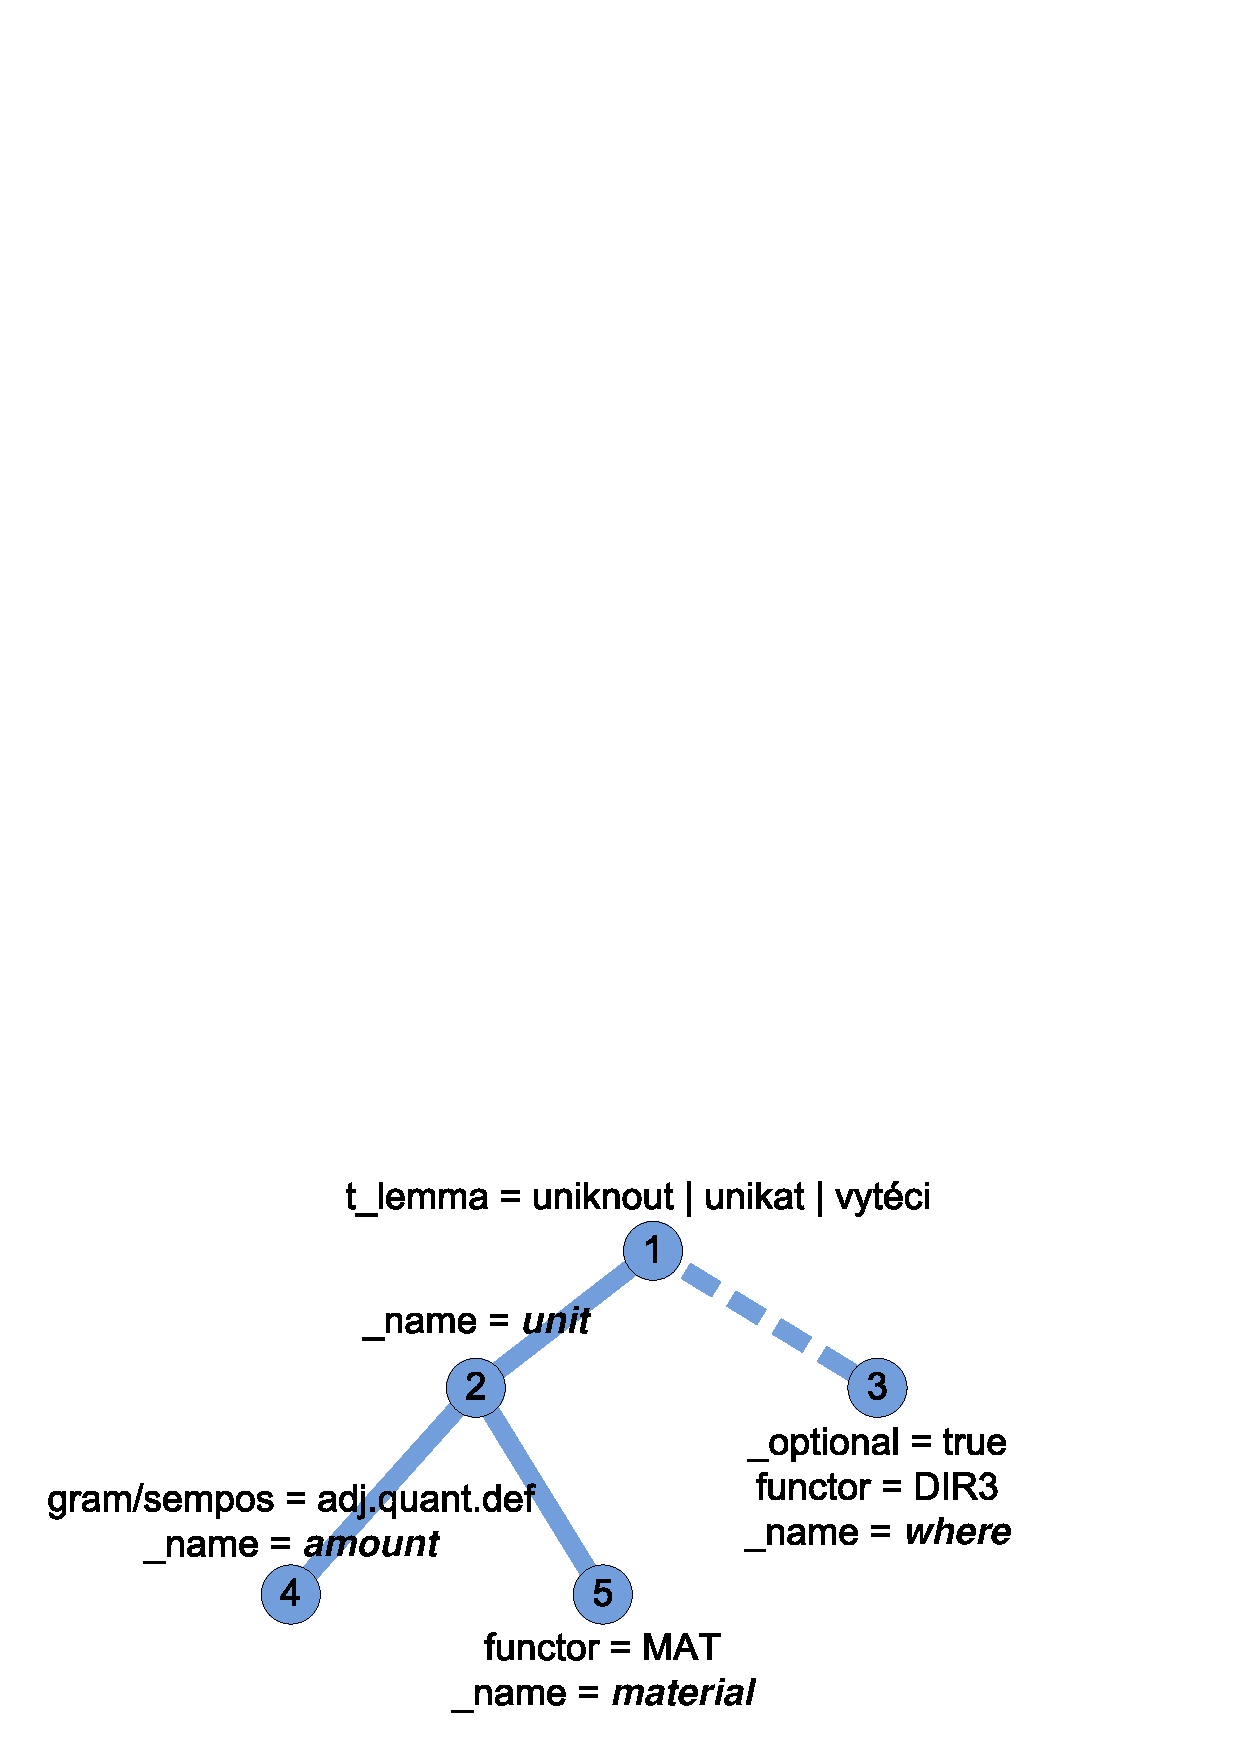
\includegraphics[width=0.5\hsize]{eenv_extract_patern}
\\Transcript:\\
\begin{tabular}{|c|c|}
\hline
uniknout, unikat & vytéci\\
to leak out & to flow out\\
\hline
\end{tabular}		
	\caption{A manually created extraction rule investigating dangerous liquids that spilled out into the environment.}
	\label{fig:ch50_eenv_extract_patern}
\end{figure}


\begin{figure}
	\centering
		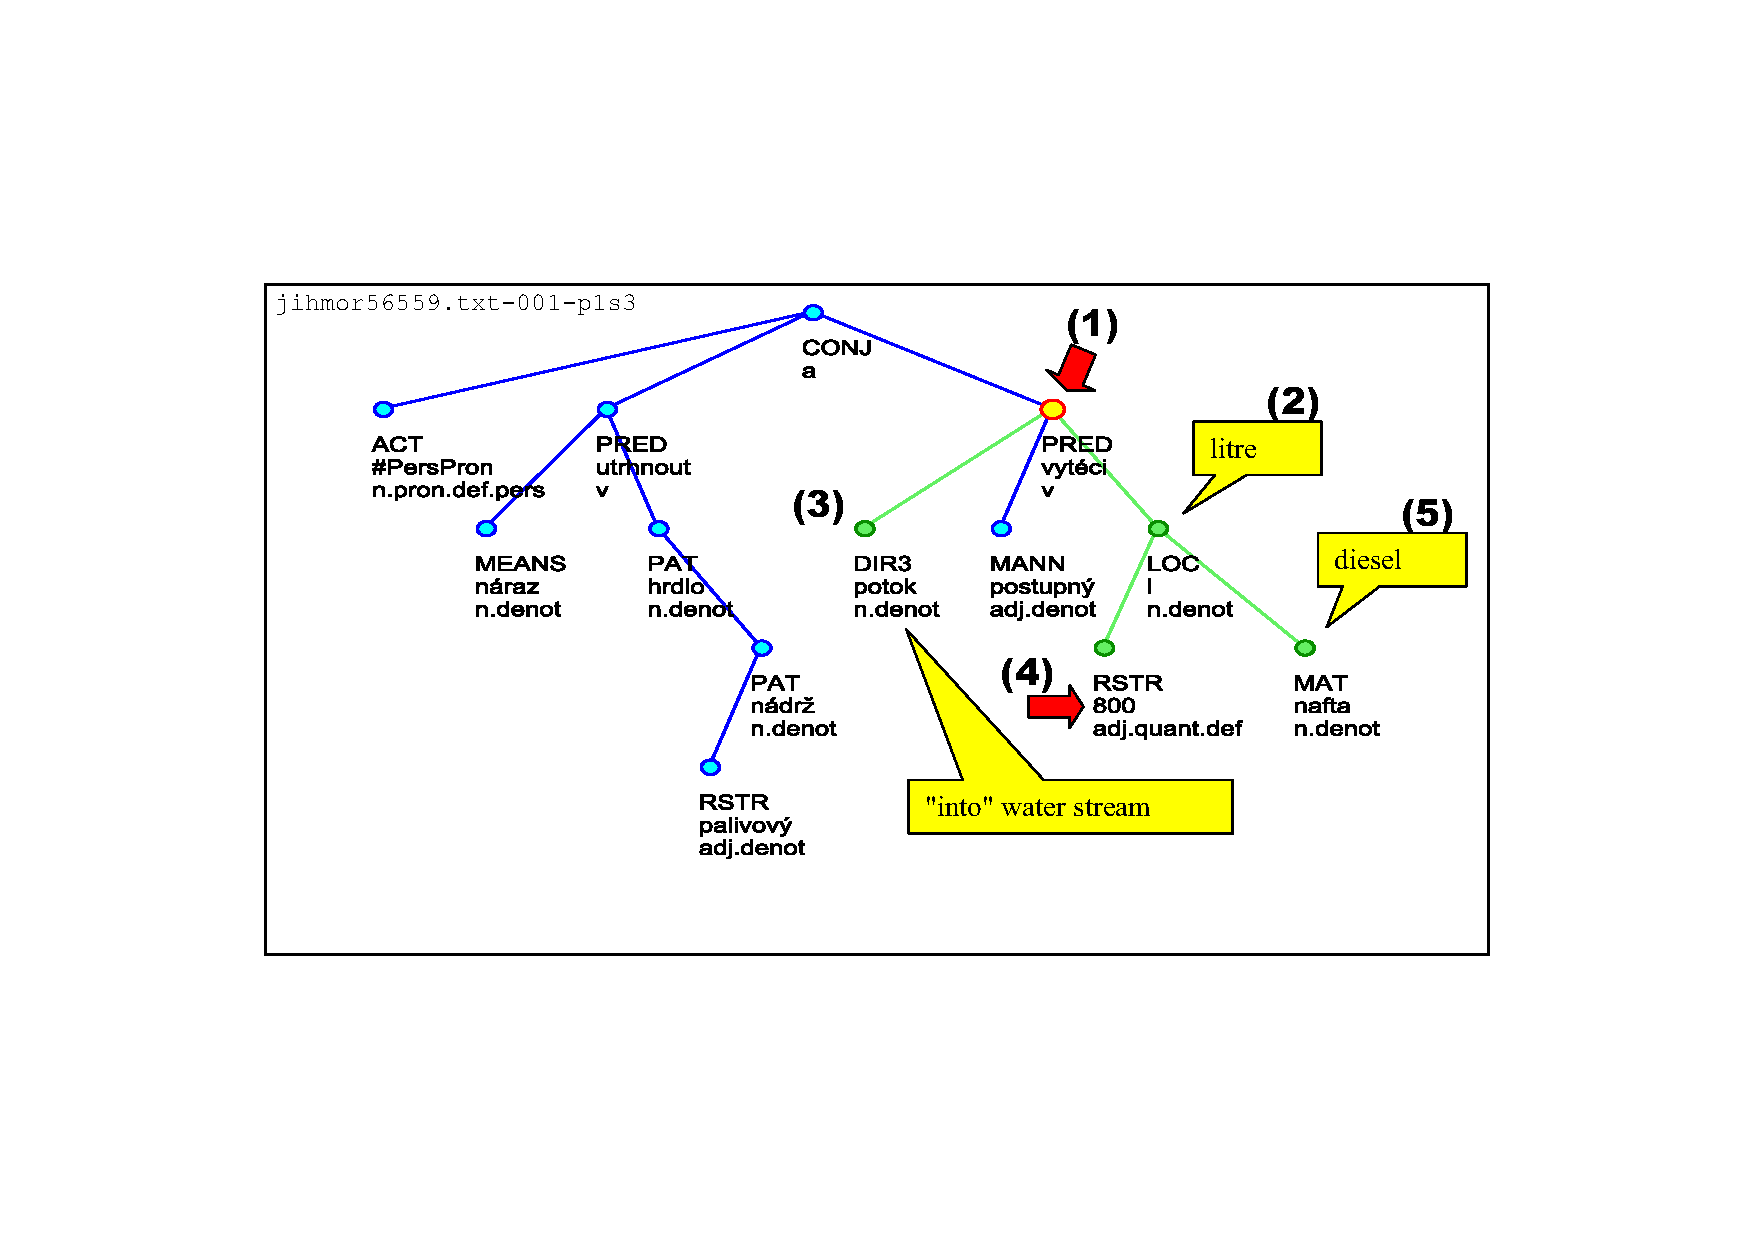
\includegraphics[angle=-90, width=0.6\hsize]{eenv_matching_tree}
		
Original sentence: 
\emph{``Nárazem se utrhl hrdlo palivové nádrže a do potoka postupně vyteklo na 800 litrů nafty.''}\\
English transcript: 
\emph{``Due to the clash the throat of fuel tank tore off and 800 liters of oil (diesel) has run out to a stream.''}
	\caption{A tree matching with the corresponding extraction rule in Figure~\ref{fig:ch50_eenv_extract_patern}.}
	\label{fig:ch50_eenv_matching_tree}
\end{figure}


%%%%%%%%%%%%%%%%%%%%%%%%%%%%%%%%%%%%%%%%%%%%%%%%%%%%%%%%%%%%%%%%%%%%%%%%%%%%%%%%%%%%%
\begin{figure}
\begin{minted}[linenos,  fontsize=\footnotesize,
               frame=lines]{xml}
<QueryMatches>
	<Match root_id="T-vysocina63466.txt-001-p1s4" match_string="2:0,7:3,8:4,11:2">
		<Sentence>
			Při požáru byla jedna osoba lehce zraněna - jednalo se
			o majitele domu, který si vykloubil rameno.
		</Sentence>
		<Data>
			<Value variable_name="action_type" attribute_name="t_lemma">zranit</Value>
			<Value variable_name="injury_manner" attribute_name="t_lemma">lehký</Value>
			<Value variable_name="participant" attribute_name="t_lemma">osoba</Value>
			<Value variable_name="quantity" attribute_name="t_lemma">jeden</Value>
		</Data>
	</Match>
	<Match root_id="T-jihomoravsky49640.txt-001-p1s4" match_string="1:0,13:3,14:4">
		<Sentence>
			Ve zdemolovaném trabantu na místě zemřeli dva muži - 82letý senior
			a další muž, jehož totožnost zjišťují policisté.
		</Sentence>
		<Data>
			<Value variable_name="action_type" attribute_name="t_lemma">zemřít</Value>
			<Value variable_name="participant" attribute_name="t_lemma">muž</Value>
			<Value variable_name="quantity" attribute_name="t_lemma">dva</Value>
		</Data>
	</Match>
	<Match root_id="T-jihomoravsky49736.txt-001-p4s3" match_string="1:0,3:3,7:1">
		<Sentence>Čtyřiatřicetiletý řidič nebyl zraněn.</Sentence>
		<Data>
			<Value variable_name="action_type" attribute_name="t_lemma">zranit</Value>
			<Value variable_name="a-negation" 
			       attribute_name="m/tag">VpYS---XR-NA---</Value>
			<Value variable_name="participant" attribute_name="t_lemma">řidič</Value>
		</Data>
	</Match>
</QueryMatches>
\end{minted}
\caption{\emph{XML} structured output of the SQL select like query. A negation can be detected from the presence of \emph{m/tag} on the line 30.}
\label{fig:select_xml}
\end{figure}
%%%%%%%%%%%%%%%%%%%%%%%%%%%%%%%%%%%%%%%%%%%%%%%%%%%%%%%%%%%%%%%%%%%%%%%%%%%%%%%%%%%%%

\begin{figure}
	\centering
		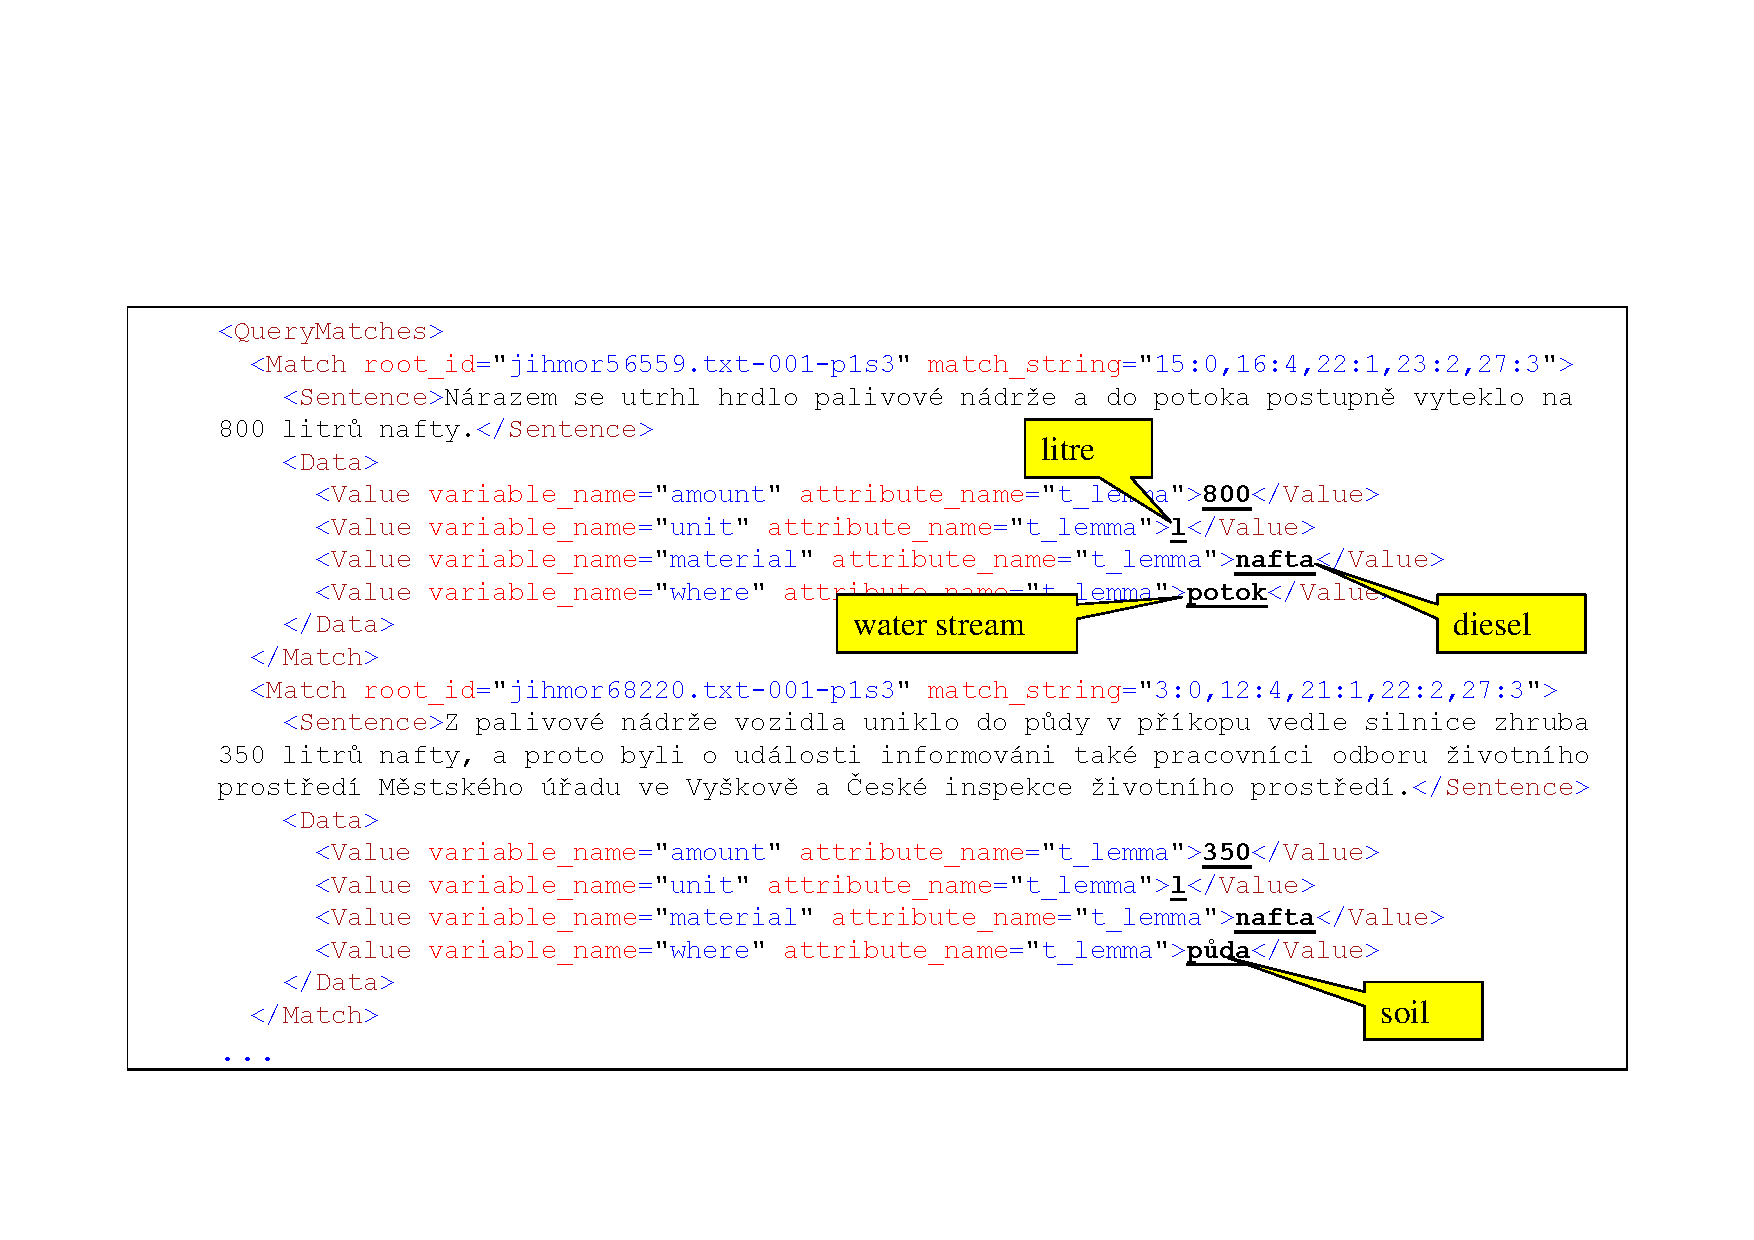
\includegraphics[angle=-90, width=0.7\hsize]{eenv_results}
	\caption{\emph{XML} structured output of the SQL select like query corresponding with the extraction rule in Figure~\ref{fig:ch50_eenv_extract_patern} and matching tree in Figure~\ref{fig:ch50_eenv_matching_tree}.}
	\label{fig:ch50_eenv_results}
\end{figure}





The second implementation was based on Netgraph -- a linguistic tool used for searching through a syntactically annotated corpus (see Section~\ref{sec:ch30_netgraph} for details). 

Netgraph queries are written in a special query language with a graphical representation. The graphical representation of a query is much better readable than its linear textual representation and in this text we will use the graphical representation only. Examples of a Netgraph queries (in the graphical representation) can be found in Figures \ref{fig:ch50_extract_patern} and \ref{fig:ch50_eenv_extract_patern}. They clearly show the necessary tree structure that has to be present in any matching tree and attribute restrictions are printed beside the corresponding nodes.

The Netgraph based extraction procedure works with extraction rules in a pseudo SQL SELECT form:

\begin{minted}{sql}
SELECT node1_name.attr1_name, node2_name.attr2_name, ... FROM netgraph_query
\end{minted}

where netgraph\_query stands for an arbitrary Netgraph query, node1\_name, node2\_name, etc. stand for individual names of nodes defined in netgraph\_query and attr1\_name, attr2\_name, etc. stand for names of linguistic attributes whose values should be picked out from the corresponding matching tree nodes.

The extraction works as follows: the Netgraph query is evaluated by searching through a corpus of linguistic trees. Matching trees are returned and the desired information defined by the SELECT part of the extraction rule is taken from particular tree nodes and printed to the output.

\subsection{Illustration Examples}

Let us explain it in more detail by using the example of extraction rule from the Figure~\ref{fig:ch50_extract_patern}, which is looking for information about killed and injured people during a (usually car) accident. This rule consists of five nodes. Each node of the rule will match with the corresponding node in each matching tree. So we can investigate the relevant information by reading values of linguistic attributes of matching nodes. We can find out the number (node number 5) and kind (4) of people, which were or were not (2) killed or injured (1) by an accident that is presented in the given sentence. And we can also identify the manner of injury (light or heavy) in the node number 3.

Evaluation of the extraction rule from Figure~\ref{fig:ch50_eenv_extract_patern} is illustrated on Figure~\ref{fig:ch50_eenv_matching_tree}. Figure~\ref{fig:ch50_eenv_matching_tree} shows a linguistic tree matching with the extraction rule. Matching nodes are decorated and labeled by the numbers of corresponding query nodes.


\subsection{Extraction Output}

Small pieces of extraction outputs are shown in Figure~\ref{fig:select_xml} (for the extraction rule in Figure~\ref{fig:ch50_extract_patern}) and in Figure~\ref{fig:ch50_eenv_results} (for the extraction rule in Figure~\ref{fig:ch50_eenv_extract_patern}). 

The former example (Figure~\ref{fig:select_xml}) contains three matches of the extraction rule in three different articles. Each query match is closed in the \verb+<Match>+ element and each contains values of some linguistic attributes closed inside the \verb+<Value>+ elements. Each value comes from some of the nodes of the extraction rule. Name of corresponding query node is saved in the \verb+variable_name+ attribute of the \verb+<Value>+ element.

In the case of the example query, values identified by the variable \verb+action_type+ specify the type of the action. So in the first and third case somebody was injured (\emph{zranit} means to injure in Czech, lines 8 and 28) and in the second case somebody died (\emph{zemřít} means to die in Czech, line 20).

Values identified by \verb+participant+ and \verb+quantity+ contain information about participants of the action. \verb+participant+ serves for specification of the type of the participants and \verb+quantity+ values hold numbers (quantity) of the participants. So in the first action one (\emph{jeden}, line 11) person (\emph{osoba}, line 10) was injured and in the second action two (\emph{dva}, line 22) men (\emph{muž}, line 21) died.

Values identified by \verb+a-negation+ contain the information about a negation of a clause (The presence of negation is indicated by the 11th character of the position-based morphological tag, note that the corresponding node (number 2) of the extraction rule is marked as optional and the restriction on m/tag is put in the form of regular expression on the 11th character.) So we can see that the participant (driver -- \emph{řidič}, line 31) of the last action was \textbf{not} injured (lines 29-30).

The last not described attribute name is \verb+injury_manner+. Corresponding values contain information about the manner of injury of an injury action. So in the first action of the example there was a light injury (\emph{lehký} means light in Czech, line 9).






%%%%%%%%%%%%%%%%%%%%%%%%%%%%%%%%%%%%%%%%%%%%%%%%%%%%%%%%%%%%%%%%%%%%%%%%%%%%%%%%%%%%%
\section{Experiments and Evaluation}
%%%%%%%%%%%%%%%%%%%%%%%%%%%%%%%%%%%%%%%%%%%%%%%%%%%%%%%%%%%%%%%%%%%%%%%%%%%%%%%%%%%%%


In this section two experiments with manually created extraction rules will be presented. The first one provides measurements on a higher amount of texts without manual gold standard annotations, while the second experiment was done on a small manually annotated collection. 

\subsection{First Experiment -- Quantitative Evaluation} \label{sec:ch50_quant_experiment}

We evaluated three extraction rules (one procedural and two Netgraph based) on a set of 814 texts of news of several Czech fire departments and measured several statics. All the rules had the same goal: to find numbers of people that died or were injured during an accident. The procedural rule was the same as in Figure~\ref{lst:btred_rule} and the Netgraph based rules correspond with the rule in Figure~\ref{fig:ch50_extract_patern}. The only difference between the Netgraph rules is that in the first case (Netgraph 1) all rule nodes except number 1 (\verb+action_type+) were set as optional, while in the second case (Netgraph 2) also node 4 (participant) was compulsory. This little change caused some interesting effects -- see below. 

Table~\ref{tab:ch50_tab_manual_rules} summarizes some of the statics that were measured. Description of individual values follows.

\begin{table}
	\centering
		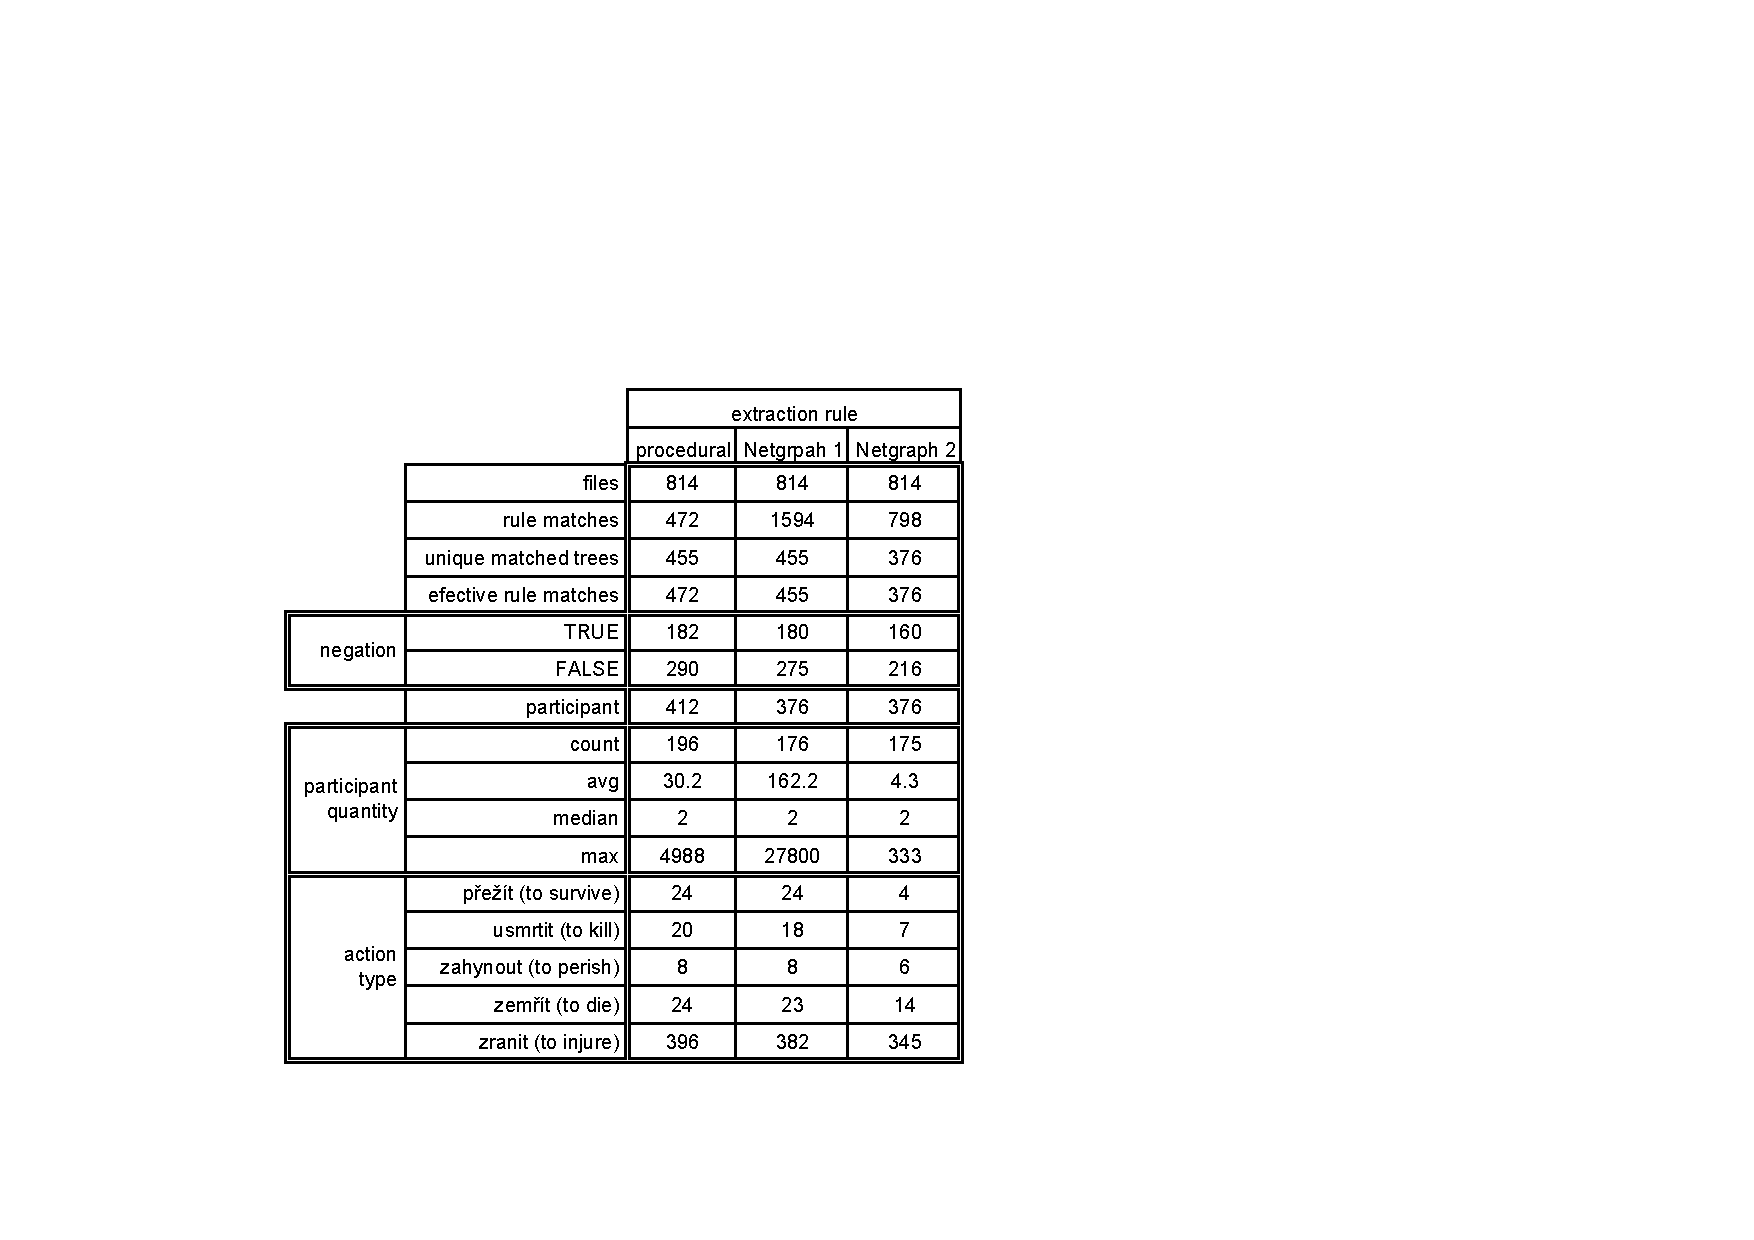
\includegraphics[angle=-90,width=0.6\hsize]{tab_manual_rules}
	\caption{Evaluation of manually created rules (bigger dataset without manual annotations).}
	\label{tab:ch50_tab_manual_rules}
\end{table}


\begin{description}
	\item[Files]
The same set of 814 files (texts) was used in all the experiments.

	\item[Rule matches]
The presence of optional nodes in a query increases the number of possibilities how a Netgraph query can be matched to a single linguistic tree. An optional node might or might not be marked in the result. The number of possible matches is also increased if there are more compatible nodes in a candidate tree that can be matched with a single query node. This can even be true for the participant query node (4) in the case of Netgraph based rules if a sentence mentions more than one affected person. This can be marked as a mistake in the rule design -- it does not count with such possibility, or it can be taken as a drawback of the current evaluation algorithm of the Netgraph based method -- it should put all the possibilities to the output. Note that this issue does not concern the procedural method, which outputs all the matching participants.

	\item[Unique matched trees]
This number represents the number of unique trees matched by the extraction rule.

	\item[Effective rule matches]
Because the procedural rules and the Netgraph based rules are evaluated in a different way, the way of selection of effective matches (matches that are used for the output) is also different. In the procedural case all matches are used because every such match is tied up with a different verb in a sentence. In this case more matches per sentence (tree) are only possible for complex sentences with more verbs and therefore every match is applicable because it is connected with a different piece of information.\\
In the Netgraph case it is necessary to select the most relevant matches of all possible ones. The first longest (maximum of optional nodes) match for each tree is selected. This is unfortunately not optimal and also not consistent with the procedural case, but it is the easiest option for the implementation (Netgraph can be directly used in that case.)

	\item[Negation, participant, participant quantity (count), action type]
These values represent numbers of matching nodes (or more precisely of pieces of extracted information) of the given type. For example values of participant are the numbers of all participants (node number 4 in the Netgraph based rule) identified by the extraction rule and values of \emph{přežít} (survive) are numbers of matching action type nodes with the value of \emph{přežít} (survive). Note that some postprocessing of the Netgraph based output was necessary to count TRUE and FLASE negation values.

	\item[Participant quantity]
Values in this group are all connected with the quantity kind of information. It expresses the quantity of participants involved in the corresponding incident action. This kind of information is numeric so some numerical calculations can be made (average value, median and maximum value). Again postprocessing of the Netgraph based output was necessary to obtain these values -- in this case translation of seven kinds of numerals to numbers (\emph{jeden} - 1, \emph{dva} - 2, \emph{tři} - 3, \emph{čtyři} - 4, \emph{šest} - 6, \emph{sedm} - 7, \emph{osm} - 8). Note that the vale of average is strongly affected by the very few high numbers present in the results (the values 1 and 2 accounted for more than half of the results.)\\
Values of participant quantity also demonstrate several errors made by the particular extraction rules, see bellow for details.
\end{description}





















\subsubsection{Detected errors}

Results of the extraction were investigated only partly; no formal evaluation is available in this case (except on a small evaluation set, see bellow: the second experiment). About 10-20\% of information was not extracted because of errors of linguistic parsing; majority of the errors was made in long complex sentences, which are known to be difficult for linguistic processing. There was only a few of false positives. A nice example can be traced from the maximum values of participant quantity in Table 99. Three different numbers were found in the three experiments: 27800, 4988 and 333. The number of 27800 is actually a number of chickens that died during one of the accidents. The number was extracted by the first Netgraph based rule because the query node 4 (participant) was marked as optional and omitted during the evaluation. This node normally ensures that the participant is one of: person, man, woman, child, driver, etc.
Numbers 4988 and 333 are both correct. They were both used in the same sentence, which summarized numbers of injured (4988) and killed (333) people during one whole year. Although the sentence was quite complex it was linguistically parsed correctly and also the procedural rule managed to extract both numbers correctly. The Netgraph based rule extracted only the first number in the sentence because the current evaluation algorithm does not allow multiple matches per sentence (see above the comments of rule matches and effective rule matches).


\subsection{Second Experiment -- Qualitative Evaluation}


\begin{table}
	\centering
	\begin{tabular}{|r|c|c|c|c|c|c|}
		\hline
		 & correct & missing & spurious & recall & precision & $F_1$\\
		\hline
		injuries & 3 & 29 & 0 & 0.09 & 1 & 0.17\\
		\hline
		fatalities & 1 & 10 & 0 & 0.09 & 1 & 0.17\\
		\hline
	\end{tabular}
	\caption{Evaluation of the manually created rule form Figure~\ref{fig:ch50_extract_patern} on the manually annotated dataset.}
	\label{tab:ch50_extract_patern_eval}
\end{table}



In the second experiment a manually annotated collection of 50 fireman news texts was used. Having the extraction rule from the previous experiment and a set of manually annotated texts it is only natural to ask a question about the success of the extraction rule on that collection. Table~\ref{tab:ch50_extract_patern_eval} summarizes the results. These results are far from satisfactory; the recall of 0.09 is something that is far from any acceptable use. Several explanations of the issue can be provided. The extraction rule serves more for a demonstration than for exhausting coverage of all possible cases. The extraction rule looks for particular verb (to injure, to die, etc.) but the information can be also expressed by an adjective (injured driver, death passenger, etc.); another extraction rules should be constructed for these and other cases. The training collection used for the design was also of a different spectrum of texts.



On the other hand this experiment shows how a manually annotated collection contributes to the quality of extraction rules. We can never know if the extraction rule is usable until a formal evaluated is made. Also the fact that the precision is strictly 1 should be noted. This means that the extraction rule made no mistake in those cases when it provided some output.



\subsubsection{Manual Design of Rules Using Training Data Set}  

\begin{table}
	\centering
	\begin{tabular}{|r|c|c|c|c|c|c|}
		\hline
		 & correct & missing & spurious & recall & precision & $F_1$\\
		\hline
		manual rules & 5 & 2 & 0 & 0.71 & 1 & 0.83\\
		\hline
		ILP rules & 5 & 2 & 0 & 0.71 & 1 & 0.83\\
		\hline
	\end{tabular}
	\caption{Evaluation of the manually created rules and ILP learned rules (manually annotated dataset was used for rule design (training half) and evaluation (testing half) -- see the description of the second experiment in text.)}
	\label{tab:ch50_damage_manual_eval}
\end{table}

\begin{table}
	\centering
	\begin{tabular}{|r|c|c|c|c|c|c|}
		\hline
		 & correct & missing & spurious & recall & precision & $F_1$\\
		\hline
		manual rules & 4 & 1 & 1 & 0.8 & 0.8 & 0.8\\
		\hline
		ILP rules & 4 & 1 & 1 & 0.8 & 0.8 & 0.8\\
		\hline
	\end{tabular}
	\caption{Cross method comparison of found instances.}
	\label{tab:ch50_damage_cross_method}
\end{table}




Next question that naturally emerges is: How would be the performance if the rules were designed with the support of a manually annotated collection? An additional experiment was made to answer that question. The collection was split into two even parts -- training part and testing part. A manually created rule was designed so that it correctly matched with all annotations of the training part and then it was evaluated on the testing part. For the validity of the experiment it was necessary that the designer did not have any knowledge about the data of the testing part; that is why we used a different extraction task (damage instead of injuries and fatalities).We have also compared the performance of the manually created rule with a rule learned by the ILP machine learning engine (see Chapter~\ref{ch:ILP_Learning}).

The results are summarized in Table~\ref{tab:ch50_damage_manual_eval}. Both kinds of rules (manually designed and learned by ILP) performed the same (recall: 0.71, precision: 1); both the methods correctly found 5 instances and they were both unable to find 2 instances. From the cross coverage comparison in 
Table~\ref{tab:ch50_damage_cross_method} it is apparent that the methods agreed on 4 instances and each method was able to discovered one instance that the other did not discover. Such results could be accepted for a practical application but we must not forget the fact that the collection is very small and only single evidence is provided by the experiment, so it dies not provide any statistical significance (getting statistically significant results would require experiments with different datasets, extraction tasks and human designers.) 



%%%%%%%%%%%%%%%%%%%%%%%%%%%%%%%%%%%%%%%%%%%%%%%%%%%%%%%%%%%%%%%%%%%%%%%%%%%%%%%%%%%%%
\section{Conclusion}
%%%%%%%%%%%%%%%%%%%%%%%%%%%%%%%%%%%%%%%%%%%%%%%%%%%%%%%%%%%%%%%%%%%%%%%%%%%%%%%%%%%%%

Note that in this case we did not concern the annotation aspect of information extraction. Although it is possible to infer an annotation based variety of the presented method, here we did not take it into account because during the development of the method the aim was more to produce structured data from text than to produce annotated documents. In the next section the emphasis will be inverted. 

A deeper evaluation of the method would be definitely interesting, but at the moment the information provided is the only available. There is no real world application of the method outside the academic ground. The method is still waiting for deep testing and further development in an extensive real world project.

